%%%%%%%%%%%%%%%%%%%%%%%%%%%%%%%%%%%%%%%%%%%%%%%%%%%%%%%%%%%%%%%%%%%%%%%%
% Uni Duesseldorf
% Lehrstuhl fuer Datenbanken und Informationssysteme
% Vorlage fuer Bachelor-/Masterarbeiten
% Optimiert fuer den Original-Latex-Kompiler LATEX.EXE (LaTeX=>PS=>PDF)
%%%%%%%%%%%%%%%%%%%%%%%%%%%%%%%%%%%%%%%%%%%%%%%%%%%%%%%%%%%%%%%%%%%%%%%%
% Ueberarbeitung für pdflatex (LaTeX=>PDF)
%%%%%%%%%%%%%%%%%%%%%%%%%%%%%%%%%%%%%%%%%%%%%%%%%%%%%%%%%%%%%%%%%%%%%%%%
% Vorlage Changelog:
% 10.09.2015 (Matthias Liebeck): Nummerierung des Inhaltsverzeichnis nun römisch, Beispiel für einen Anhang eingebaut, \raggedbottom hinter sections eingefügt
% 11.07.2018 (Matthias Liebeck): Ersetzung des Bibliographiestils, Einsatz von Biber
% 04.09.2018 (Matthias Liebeck):
%   * Bibtex: unnötige Bibtexfelder beim Rendern ausblenden (thx @ Markus Brenneis)
%   * ngerman: "et al." im BibTeX für drei oder mehr Autoren
%   * Neuer Befehl \sectionforcestartright: Sections immer rechts beginnen (thx @ Philipp Grawe)
%   * ngerman: Deutsche Anführungszeichen im Literaturverzeichnis (thx @ Markus Brenneis)
%   * ngerman: Deutsche Anführungszeichen im Literaturverzeichnis (thx @ Markus Brenneis)
% 16.10.2018 (Matthias Liebeck): Zwei fixes an \sectionforcestartright (thx @ Markus Brenneis)
%%%%%%%%%%%%%%%%%%%%%%%%%%%%%%%%%%%%%%%%%%%%%%%%%%%%%%%%%%%%%%%%%%%%%%%%
%%%% BEGINN EINSTELLUNG FUER DIE ARBEIT. UNBEDINGT ERFORDERLICH! %%%%%%%
%%%%%%%%%%%%%%%%%%%%%%%%%%%%%%%%%%%%%%%%%%%%%%%%%%%%%%%%%%%%%%%%%%%%%%%%
% Geben Sie Ihren Namen hier an:
\raggedbottom
\newcommand{\bearbeiter}{Hanna Pankova}

% Geben Sie hier den Titel Ihrer Arbeit an:
\newcommand{\titel}{AI-based fluorescent labeling for cell line development}

% Geben Sie das Datum des Beginns und Ende der Bachelorarbeit ein:
\newcommand{\beginndatum}{01. April 2022}
\newcommand{\abgabedatum}{29. August 2022}

% Geben Sie die Namen des Erst- und Zweitgutachters an:
\newcommand{\erstgutachter}{Prof. Dr. Markus Kollmann}
\newcommand{\zweitgutachter}{Dr. Wolfgang Halter}

% Falls Sie die Arbeit zweiseitig ausdrucken wollen,
% benutzen Sie die folgende Zeile mit
% \AN fuer zweiseitigen Druck
% \AUS fuer einseitigen Druck
\newcommand{\zweiseitig}{\AN}
% true fuer biber, false fuer klassischen Zitierstil
%\newcommand{\biber}{false}
\newcommand{\biber}{true}

% Falls Sections immer rechts beginnen sollen. Gerade für Masterarbeiten
% interessant. Bei kurzen Bachelorarbeiten eher weniger zu verwenden.
\newcommand{\sectionforcestartright}{false}
%\newcommand{\sectionforcestartright}{true}

% Falls die Arbeit in englischer Sprache verfasst
% werden soll, dann benutzen Sie die folgende Zeile mit
% englisch fuer englische Sprache
% deutsch fuer deutsche Sprache
\newcommand{\sprache}{englisch}

% Hier wird eingestellt, ob es sich bei der Arbeit um eine Bachelor-
% oder Masterarbeit handelt (unpassendes auskommentieren!):
\newcommand{\arbeit}{Master thesis}
%~ \newcommand{\arbeit}{Masterarbeit}


%%%%%%%%%%%%%%%%%%%%%%%%%%%%%%%%%%%%%%%%%%%%%%%%%%%%%%%%%%%%%%%%%%%%%%%%
%%%% ENDE EINSTELLUNGEN %%%%%%%%%%%%%%%%%%%%%%%%%%%%%%%%%%%%%%%%%%%%%%%%
%%%%%%%%%%%%%%%%%%%%%%%%%%%%%%%%%%%%%%%%%%%%%%%%%%%%%%%%%%%%%%%%%%%%%%%%

% Die folgende Zeile NICHT EDITIEREN oder loeschen


%%%%%%%%%%%%%%%%%%%%%%%%%%%%%%%%%%%%%%%%%%%%%%%%%%%%%%%%%%%
% Obere Titelmakros. Editieren Sie diese Datei nur, wenn
% Sie sich ABSOLUT sicher sind, was Sie da tun!!!
% (Z.B. zum Abaendern der BA-Vorlage in eine MA-Vorlage)
% Uni Duesseldorf
% Lehrstuhl fuer Datenbanken und Informationssysteme
% Version 2.2 - 2.3.2010
%%%%%%%%%%%%%%%%%%%%%%%%%%%%%%%%%%%%%%%%%%%%%%%%%%%%%%%%%%%
\newcommand{\AN}{twoside}
\newcommand{\AUS}{}


%\newcommand{\englisch}{}
%\newcommand{\deutsch}{\usepackage[german]{babel}}

%% Die folgenden auskommentierten Optionen dienen der automatischen
%% Erkennung des Latex-Kompilers und dem Setzen der davon abhängigen
%% Einstellungen. Bei Problem z.B. mit dem Einbinden von verschiedenen
%% Grafiktypen bei Verwendung von PdfLatex oder Latex, einfach die
%% verschiedenen \usepackage(s) ausprobieren. (Mit diesen Einstellungen
%% funktionierte diese Vorlage bei der Verwenundg von latex.exe als
%% Kompiler bei den meisten Studierenden.)

%\newif\ifpdf \ifx\pdfoutput\undefined
%\pdffalse % we are not running pdflatex
%\else
%\pdfoutput=1 % we are running pdflatex
%\pdfcompresslevel=9 % compression level for text and image;
%\pdftrue \fi

\documentclass[11pt,a4paper, \zweiseitig]{article}
\usepackage{ifthen}


%\usepackage[iso]{umlaute}
\usepackage[utf8]{inputenc}
\usepackage{palatino} % palatino Schriftart
%\usepackage{makeidx} % um ein Index zu erstellen
\usepackage[nottoc]{tocbibind}
\usepackage[T1]{fontenc} %fuer richtige Trennung bei Umlauten
\usepackage{fancybox} % fuer die Rahmen
\usepackage{shortvrb}
\usepackage{url}
\usepackage{xcolor}
\usepackage[colorlinks,citecolor=blue,linkcolor=black]{hyperref} %anklickbares Inhaltsverzeichnis

\ifthenelse{\boolean{\biber}}{
  % only needed for biber
  \usepackage[style=authoryear,natbib=true,backend=biber,mincitenames=1,maxcitenames=2,maxbibnames=99,uniquelist=false,dashed=false]{biblatex}

  % https://tex.stackexchange.com/a/334703/8850
  \AtEveryBibitem{%
    \clearfield{issn}
    \clearfield{isbn}
    \clearfield{doi}
    \clearfield{location}
    \clearlist{location}
    \clearlist{address}

    \ifentrytype{online}{}{% Remove url except for @online
      \clearfield{url}
    }
  }
}
{}%no else

% Falls es bei \citet ein Komma zwischen Name und Jahr gibt:
% https://tex.stackexchange.com/questions/312539/unwanted-comma-between-author-and-year-using-citet-command
% (thx @ Markus Brenneis)
%\DeclareDelimFormat[cbx@textcite]{nameyeardelim}{\addspace}



\ifthenelse{\equal{\sprache}{deutsch}}{
  \usepackage[ngerman]{babel}
  % Bibtex u.a -> et al.
  \ifthenelse{\boolean{\biber}}{
    \DefineBibliographyStrings{ngerman}{
      andothers = {{et\,al\adddot}},
    }
    \newcommand{\references}{Literatur}
  }
  {} % do nothing when not using biber
  \usepackage[autostyle, german=quotes]{csquotes} % Deutsche Anführungszeichen im Literaturverzeichnis (thx @ Markus Brenneis)

}{ \newcommand{\references}{References}}

\usepackage{a4wide} % ganze A4 Weite verwenden



%\ifpdf
%\usepackage[pdftex,xdvi]{graphicx}
%\usepackage{thumbpdf} %thumbs fuer Pdf
%\usepackage[pdfstartview=FitV]{hyperref} %anklickbares Inhaltsverzeichnis
%\else
%\usepackage[dvips,xdvi]{graphicx}
\usepackage{graphicx}

%\fi

\newcommand{\redt}[1] {
  \textcolor{red}{#1}}

\newcommand{\oranget}[1] {
  \textcolor{orange}{#1}}

\newcommand{\purplet}[1] {
  \textcolor{purple}{#1}}

%%%%%%%%%%%%%%%%%%%%%%% Massangaben fuer die Arbeit %%%%%%%%%%%%%%%
\setlength{\textwidth}{15cm}

\setlength{\oddsidemargin}{35mm}
\setlength{\evensidemargin}{25mm}

\addtolength{\oddsidemargin}{-1in}
\addtolength{\evensidemargin}{-1in}

\ifthenelse{\boolean{\biber}}{\addbibresource{references.bib}}{}

%\makeindex
\begin{document}
%\setcounter{secnumdepth}{4} %Nummerieren bis in die 4. Ebene
%\setcounter{tocdepth}{4} %Inhaltsverzeichnis bis zur 4. Ebene

\pagestyle{headings}

\sloppy % LaTeX ist dann nicht so streng mit der Silbentrennung
%~ \MakeShortVerb{\§}

\parindent0mm
\parskip0.5em


{
\textwidth170mm
\oddsidemargin30mm
\evensidemargin30mm
\addtolength{\oddsidemargin}{-1in}
\addtolength{\evensidemargin}{-1in}

\parskip0pt plus2pt

% Die Raender muessen eventuell fuer jeden Drucker individuell eingestellt
% werden. Dazu sind die Werte fuer die Abstaende `\oben' und `\links' zu
% aendern, die von mir auf jeweils 0mm eingestellt wurden.

%\newlength{\links} \setlength{\links}{10mm}  % hier abzuaendern
%\addtolength{\oddsidemargin}{\links}
%\addtolength{\evensidemargin}{\links}

\begin{titlepage}
\vspace*{-1.5cm}
\raisebox{17mm}{
    \begin{minipage}[t]{70mm}
        \begin{center}
            %\selectlanguage{german}
            {\Large INSTITUTE OF COMPUTER SCIENCES\\}
            {\normalsize
                Master in Artificial Intelligence and Data Science\\
            }
            \vspace{3mm}
            {\small Universitätsstr. 1 \hspace{5ex} D--40225 Düsseldorf\\}
        \end{center}
    \end{minipage}
}
\hfill
\raisebox{7mm}{
    
\includegraphics[width=130pt]{bilder/HHU_Logo}}
\vspace{14em}

% Titel
\begin{center}
    \baselineskip=55pt
    \textbf{\huge \titel}
    \baselineskip=0 pt
\end{center}

%\vspace{7em}

\vfill

% Autor
\begin{center}
    \textbf{\Large
        \bearbeiter
    }
\end{center}

\vspace{35mm}

% Prüfungsordnungs-Angaben
\begin{center}
%\selectlanguage{german}

%%%%%%%%%%%%%%%%%%%%%%%%%%%%%%%%%%%%%%%%%%%%%%%%%%%%%%%%%%%%%%%%%%%%%%%%%
% Ja, richtig, hier kann die BA-Vorlage zur MA-Vorlage gemacht werden...
% (nicht mehr nötig!)
%%%%%%%%%%%%%%%%%%%%%%%%%%%%%%%%%%%%%%%%%%%%%%%%%%%%%%%%%%%%%%%%%%%%%%%%%
{\Large \arbeit}

\vspace{2em}
\ifthenelse{\equal{\sprache}{deutsch}}{
    \begin{tabular}[t]{ll}
    Beginn der Arbeit:& \beginndatum \\
    Abgabe der Arbeit:& \abgabedatum \\
    Gutachter:         & \erstgutachter \\
    & \zweitgutachter \\
}{
    \begin{tabular}[t]{ll}
    Date of issue:& \beginndatum \\
    Date of submission:& \abgabedatum \\
    Reviewers:         & \erstgutachter \\
    & \zweitgutachter \\
}
\end{tabular}
\end{center}

\end{titlepage}

}

%%%%%%%%%%%%%%%%%%%%%%%%%%%%%%%%%%%%%%%%%%%%%%%%%%%%%%%%%%%%%%%%%%%%%
\clearpage
\begin{titlepage}
    ~                % eine leere Seite hinter dem Deckblatt
\end{titlepage}
%%%%%%%%%%%%%%%%%%%%%%%%%%%%%%%%%%%%%%%%%%%%%%%%%%%%%%%%%%%%%%%%%%%%%
\clearpage
\begin{titlepage}
    \vspace*{\fill}

    \section*{Erklärung}

    %%%%%%%%%%%%%%%%%%%%%%%%%%%%%%%%%%%%%%%%%%%%%%%%%%%%%%%%%%%
    % Und hier ebenfalls ggf. BA durch MA ersetzen...
    % (Auch nicht mehr nötig!)
    %%%%%%%%%%%%%%%%%%%%%%%%%%%%%%%%%%%%%%%%%%%%%%%%%%%%%%%%%%%

    Hiermit versichere ich, dass ich diese \arbeit{}
    selbstständig verfasst habe. Ich habe dazu keine anderen als die
    angegebenen Quellen und Hilfsmittel verwendet.

    \vspace{25 mm}

    \begin{tabular}{lc}
        Düsseldorf, den \abgabedatum \hspace*{2cm} & \underline{\hspace{6cm}} \\
                                                   & \bearbeiter
    \end{tabular}

    \vspace*{\fill}
\end{titlepage}

%%%%%%%%%%%%%%%%%%%%%%%%%%%%%%%%%%%%%%%%%%%%%%%%%%%%%%%%%%%%%%%%%%%%%
% Leerseite bei zweiseitigem Druck
%%%%%%%%%%%%%%%%%%%%%%%%%%%%%%%%%%%%%%%%%%%%%%%%%%%%%%%%%%%%%%%%%%%%%

\ifthenelse{\equal{\zweiseitig}{twoside}}{\clearpage\begin{titlepage}
        ~\end{titlepage}}{}

%%%%%%%%%%%%%%%%%%%%%%%%%%%%%%%%%%%%%%%%%%%%%%%%%%%%%%%%%%%%%%%%%%%%%
\clearpage
\begin{titlepage}

    %%% Die folgende Zeile nicht ändern!
\section*{\ifthenelse{\equal{\sprache}{deutsch}}{Abstract}{Abstract}}
%%% Zusammenfassung:
Cell line development is an expensive and time-consuming process, however that is the most modern approach for producing the proteins needed in various pharmaceuticals.


    %%%%%%%%%%%%%%%%%%%%%%%%%%%%%%%%%%%%%%%%%%%%%%%%
    % Untere Titelmakros. Editieren Sie diese Datei nur, wenn Sie sich
    % ABSOLUT sicher sind, was Sie da tun!!!
    %%%%%%%%%%%%%%%%%%%%%%%%%%%%%%%%%%%%%%%%%%%%%%%
    \vspace*{\fill}
\end{titlepage}

%%%%%%%%%%%%%%%%%%%%%%%%%%%%%%%%%%%%%%%%%%%%%%%%%%%%%%%%%%%%%%%%%%%%%
% Leerseite bei zweiseitigem Druck
%%%%%%%%%%%%%%%%%%%%%%%%%%%%%%%%%%%%%%%%%%%%%%%%%%%%%%%%%%%%%%%%%%%%%
\ifthenelse{\equal{\zweiseitig}{twoside}}
{\clearpage\begin{titlepage}~\end{titlepage}}{}
%%%%%%%%%%%%%%%%%%%%%%%%%%%%%%%%%%%%%%%%%%%%%%%%%%%%%%%%%%%%%%%%%%%%%
\clearpage \setcounter{page}{1}
\pagenumbering{roman}
\setcounter{tocdepth}{2}
\tableofcontents

%\enlargethispage{\baselineskip}
\clearpage
%%%%%%%%%%%%%%%%%%%%%%%%%%%%%%%%%%%%%%%%%%%%%%%%%%%%%%%%%%%%%%%%%%%%%
% Leere Seite, falls Inhaltsverzeichnis mit ungerader Seitenzahl und
% doppelseitiger Druck
%%%%%%%%%%%%%%%%%%%%%%%%%%%%%%%%%%%%%%%%%%%%%%%%%%%%%%%%%%%%%%%%%%%%%
\ifthenelse{ \( \equal{\zweiseitig}{twoside} \and \not \isodd{\value{page}} \)}
{\pagebreak \thispagestyle{empty} \cleardoublepage}{\clearpage}


% Kapitel soll bei doppelseitigem Druck immer auf der rechten (ungeraden) Seite anfangen (thx @ Philipp Grawe)
% https://tex.stackexchange.com/a/223387
\ifthenelse{\boolean{\sectionforcestartright}}
{\let\oldsection\section % Store \section in \oldsection
    \renewcommand{\section}{\cleardoublepage\oldsection}}
{}
\pagenumbering{arabic}
\setcounter{page}{1}

%%%%%%%%%%%%%%%%%%%%%%%%%%%%%%%%%%%%%%%%%%%%%%%%%%%%%%%%%%%%%%%%%%%%%%%%
%%%% BEGINN TEXTTEIL %%%%%%%%%%%%%%%%%%%%%%%%%%%%%%%%%%%%%%%%%%%%%%%%%%%
%%%%%%%%%%%%%%%%%%%%%%%%%%%%%%%%%%%%%%%%%%%%%%%%%%%%%%%%%%%%%%%%%%%%%%%%

%%%%%%%%%%%%%%%%%%%%%%%%%%%%%%%%%%%%%%%%%%%%%%%%%%%%%%%%%%%%%%%%%%%%%%%%
% Text entweder direkt hier hinein schreiben oder, im Sinne der
% besseren Uebersichtlich- und Bearbeitbarkeit mittels \input die
% einzelnen Textteile hier einbinden.
%%%%%%%%%%%%%%%%%%%%%%%%%%%%%%%%%%%%%%%%%%%%%%%%%%%%%%%%%%%%%%%%%%%%%%%%

\section{Introduction}
\subsection{Motivation}
\subsection{Notation}
\section{Background}
\subsection{Biology}
Cell line development is a process of generating single cell-derived clones that produce high and consistent levels of target therapeutic protein. (pharma.lonza.com/offerings/mammalian/cell-line-development)

Differential interference contrast (DIC) microscopy is an optical microscopy technique used to enhance the contrast in unstained, transparent samples (wikipedia).

Proteins are large biomolecules and macromolecules that comprise one or more long chains of amino acid residues (https://en.wikipedia.org/wiki/Protein).

Fluorescent labelling is the process of covalently binding fluorescent dyes to biomolecules such as nucleic acids or proteins so that they can be visualized by fluorescence imaging (https://www.nature.com/subjects/fluorescent-labelling). A fluorophore is a chemical compound that can reemit light at a certain wavelength.These compounds are a critical tool in biology because they allow experimentalists toimage particular components of a given cell in detail. (O'reilly life sciences p113)

Cell line development (CLD) is the process by which the cellular machinery is co-opted to manufacture therapeutic biologics or other proteins of interest. One can use different expression systems for cell line development: bacterial, plant-based, yeast, mammalian. (copy paste from https://www.beckman.de/resources/product-applications/lead-optimization/cell-line-development) Chinese hamster ovary (CHO) cells are the most popular mammalian cells used for protein production. (doi:10.1016/B978-0-08-100623-8.00007-4) 

First step of CLD is the
introduction of the gene of interest (GOI or a DNA vector) to CHO cells. This process is called a transfection. It is important to transfect a GOI into an optimal site of genome to secure a high protein expression over time during protein production, however pratically transfection mostly results in a vector being inserted into a random site within a host cell genome. In case the gene was transfected in the inactive site of genome (and the majority of genome is not transriptionally active) the cell will likely not express the gene. (doi:10.1016/B978-0-08-100623-8.00007-4) (doi:10.1016/j.coche.2018.08.002)

The second step is the selection of cell pools that have successful and stable gene integrations. The reasond why not all of them are suitable for cloning is the following: during the transfection only 80\% of cells recieve the vector of GOI (doi:10.1016/B978-0-08-100623-8.00007-4), only the small percent of which actually integrate a vector into the genome and, as mentioned above, only a fraction of those cells are able to stabily express a protein. (Reference needed). Such selection could be done with bulk sorting algorithm. (doi:10.1016/B978-0-08-100623-8.00007-4)

The third step in CLD is to clone the cells. The chosen stable pools of cells are phenotypically and genetically diverse - meaning they have different growth rates, metabolic profile and etc. This is not ideal for industrial production - all the cells used for protein production should be derived from the same clone ([25] here doi:10.1016/B978-0-08-100623-8.00007-4). In order to choose single best cells for further cloning one asseses several parameters like cell size, granularity, cell surface protein expression and etc. This can be done with Fluorescent Activated Cell Sorting (FACS) technology. (https://doi.org/10.1517/14712598.4.11.1821). Unfortunately fluorescence labeling is expensive and may ruin the cell due to its phototoxicity (https://doi.org/10.1371/journal.pone.0007497). There is a limited number of available fluorescent channels in microscopes as well as such labels can also be inconsistent, depend a lot on reagent quality, and require many hours of lab work. Therefore there exists a need for flurescent labeling in silico - without intervening into the cell. 

Once the cells are cloned, phenotypical and genetical heterogeneity is reduced, the next step is to charaterize clonally-derived cells based on the following criteria: cell size, growth rate, protein quality, titer, metabolities and etc. With this one can estimate clones productivity and titer. Such observations may take up to 90 days after which one can determine which cells are stable and therefore suitable for production. This is the last step of CLD process and consumes a lot of time and maintaining costs for feeding and cloning the cells. Predicting the stability of the cells directly from DIC images would reduce this time significantly allowing to escape this process completely.

However there are also some disadtantages of this approach. First, it can be less accurate than skilled cells staining perfomed manually. Extreme or unsual clones and phenotypes might be challenging if they were not used in the training set of images.

\subsection{Imaging}
The microscope used in the experiments takes photos of the well plate in random locations. The reason for that hides in the focusing problem, to get a reasonably good photo without blur it has to focus on a specific location, this is done there automatically, therefore the location of the focus is almost random. Although it might be problematic in the following sense: photos takes by the microscope in such manner do not gurantee that the focus will land in distinct spots all the time. This means that some cells taken during one of the photos might appear in the later ones. Since the photos have a high-resolution the crops are first performed and it might happen that same cell might appear in several crops. Afterwards, when crops are split between train, test and validation datasets it might happen that the same cell will once land in the train set and another time in the validation set, which will lead to a not completely fair and representative validaiton loss during training.

\subsection{ML}
Background on Unet and ML in general

Convoutional neural network is a neural network that is based on convolutional layers. It is a powerful tool for image processing and is used in medical imaging. Convolution is a linear operation used in convolutional layers that can be performed by applying a kernel (a 2d matrix) across a bigger input matrix called tensor, which can be 3d. Element-wise product between them is calculated and summed, this value will be an element of the output 2d matrix. Kernel slides accross all locations of the input tensor. In case if several different kernels were used then a 3d tensor will be created. 

Main advantage of convolutional neural networks if weight sharing. Kernel has learnable weights however these weights are shared across all locations of the kernel on the input tensor, thic strongly reduces the number of parameters needed.

CNNs also uses non-linearities like RELU, ELU, Tahn, Sigmoids and etc. They are also often combined with max pooling layers and dropouts to escape overfitting. 

Overfitting is one of the most often problems in deep learning that prevents model to generalize well for unseen data. This can happen when the model is too big for the amount of training data given, it was not regularized well or there is just not enough data for training. 

U-Net architecture is widely used for segmentation purposes. It is a convolutional neural network with the following architecture: [img] . It first performs image downsampling and upsampling afterwards.
[https://arxiv.org/pdf/1505.04597.pdf] The following architecture have been used for nuclei prediction. 
\begin{figure}[htb]
	\begin{center}
		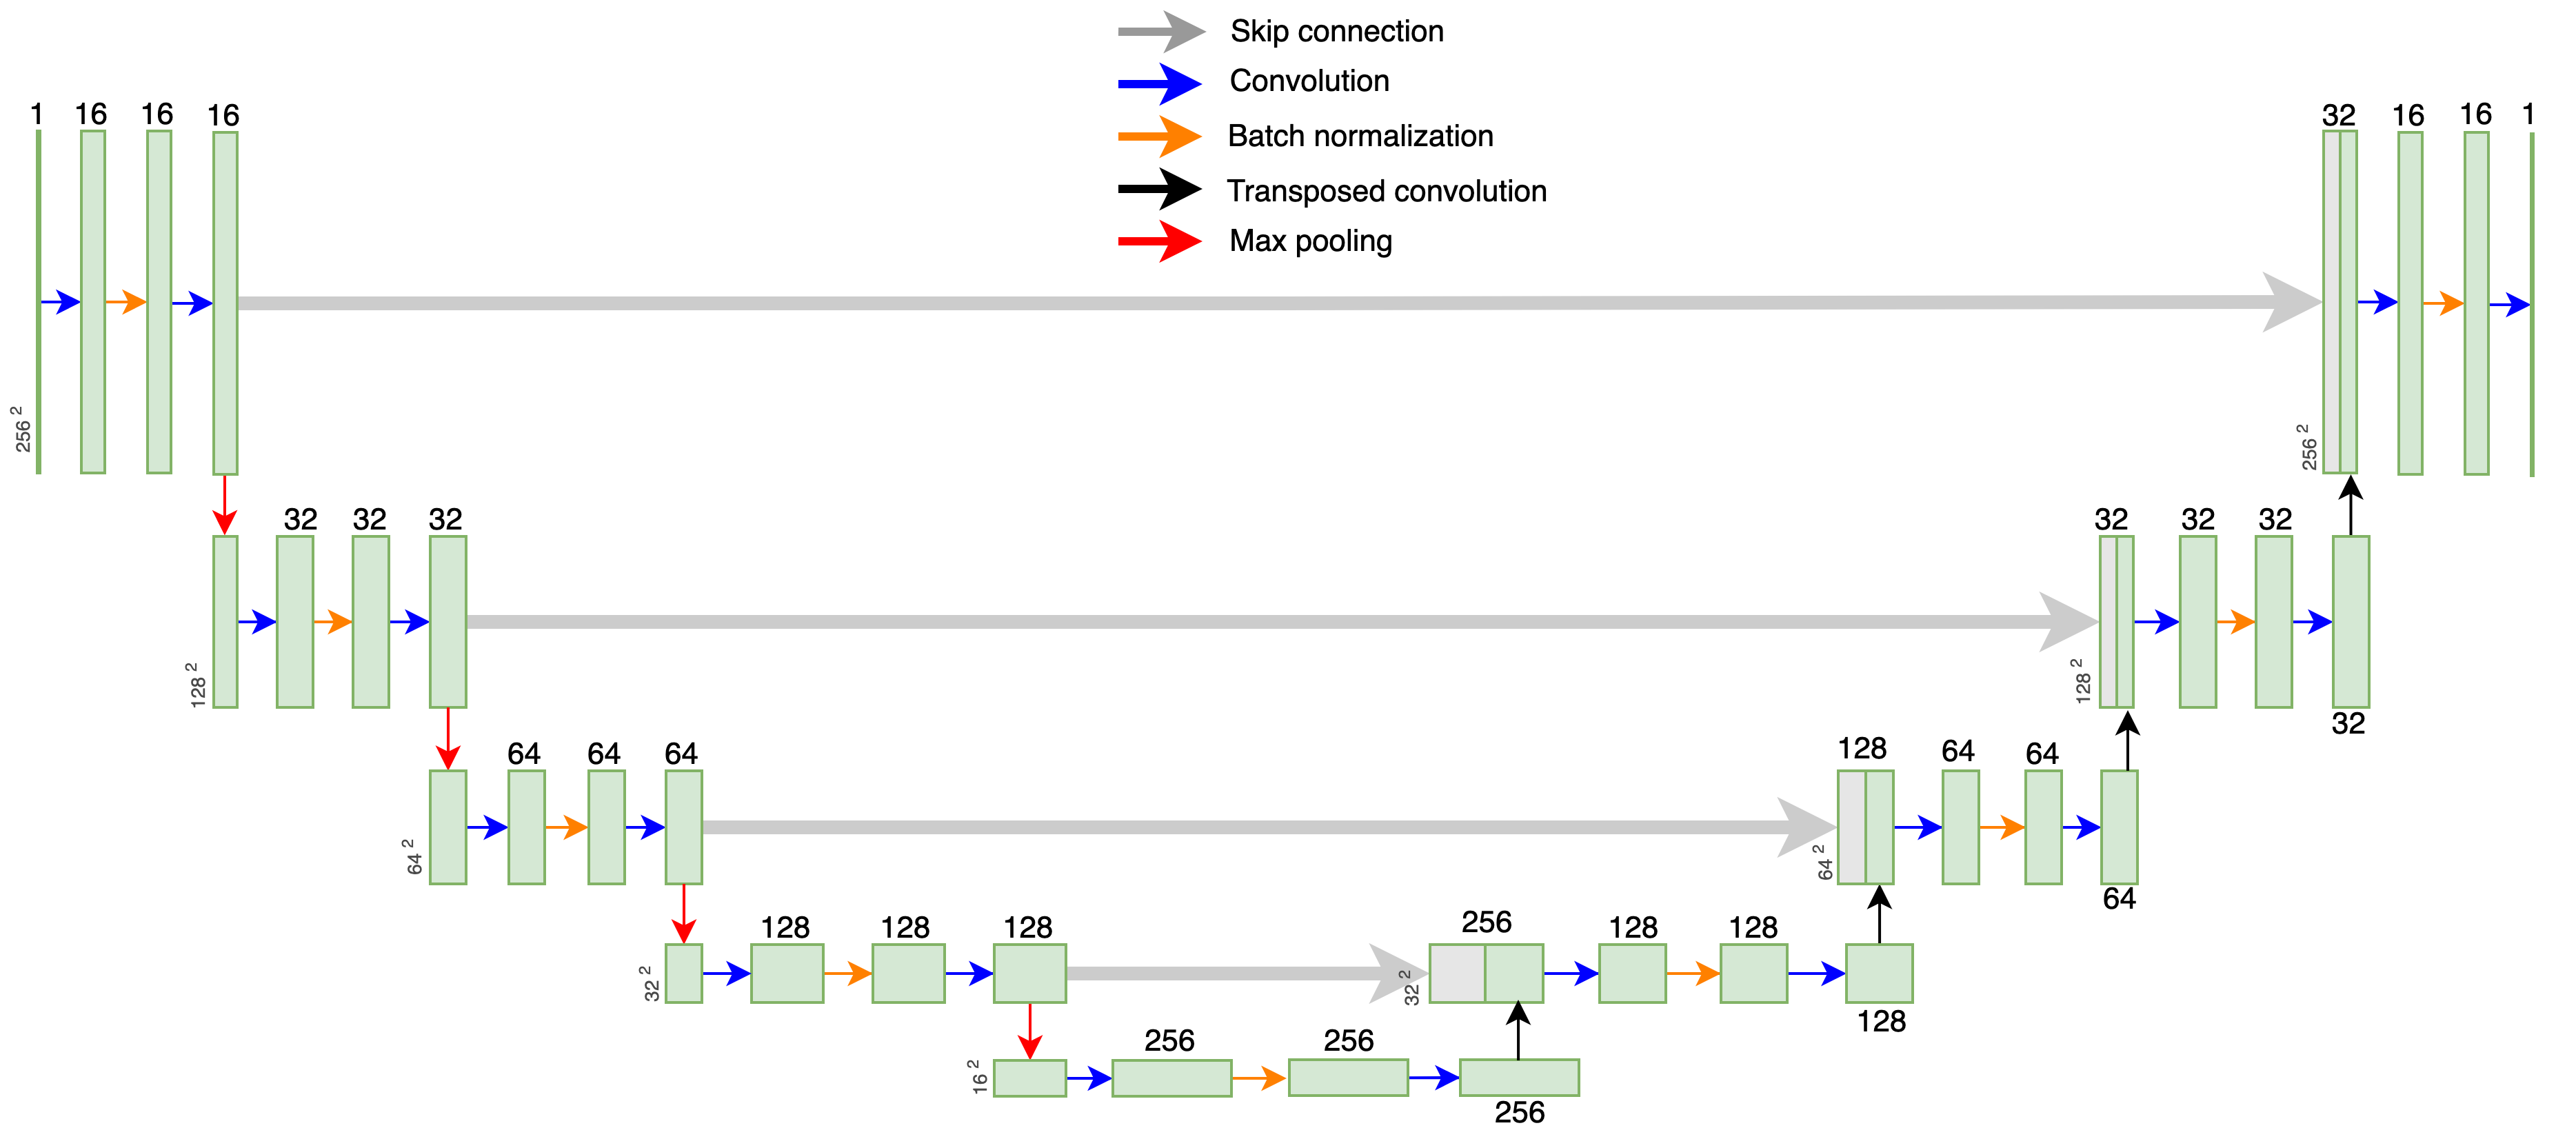
\includegraphics[width=\linewidth]{bilder/Unet.png}
		\caption{Unet}\label{fig:unet}
	\end{center}
\end{figure}

\ifthenelse{\boolean{\biber}}{ % Beispiel um mit Biber zu zitieren (\citet und \citep)
	\citet{Con97} hat ein Buch geschrieben. Es gibt auch andere Arbeiten \citep{PeHe97} die referenziert sind. In Abbildung \ref{fig_Gallien} ist ein Sachverhalt dargestellt.


	1 Autor: \citet{Con97} \hspace*{1cm} \citep{Con97}\\
	2 Autoren: \citet{IWNLP} \hspace*{1cm} \citep{IWNLP}\\
	3 Autoren: \citet{liebeck-esau-conrad:2016:ArgMining2016} \hspace*{1cm} \citep{liebeck-esau-conrad:2016:ArgMining2016}

	Online resource: \citet{ILSVRC2016}
}{ %  Beispiel um klassisch zu zitieren (\cite)
	\cite{Con97} hat ein Buch geschrieben. Es gibt auch andere Arbeiten \cite{PeHe97} die referenziert sind. In Abbildung \ref{fig_Gallien} ist ein Sachverhalt dargestellt.


	1 Autor: \cite{Con97} \hspace*{1cm} \cite{Con97}\\
	2 Autoren: \cite{IWNLP} \hspace*{1cm} \cite{IWNLP}\\
	3 Autoren: \cite{liebeck-esau-conrad:2016:ArgMining2016} \hspace*{1cm} \cite{liebeck-esau-conrad:2016:ArgMining2016}

	Online resource: \cite{ILSVRC2016}
}

\begin{figure}[htb]
	\begin{center}
		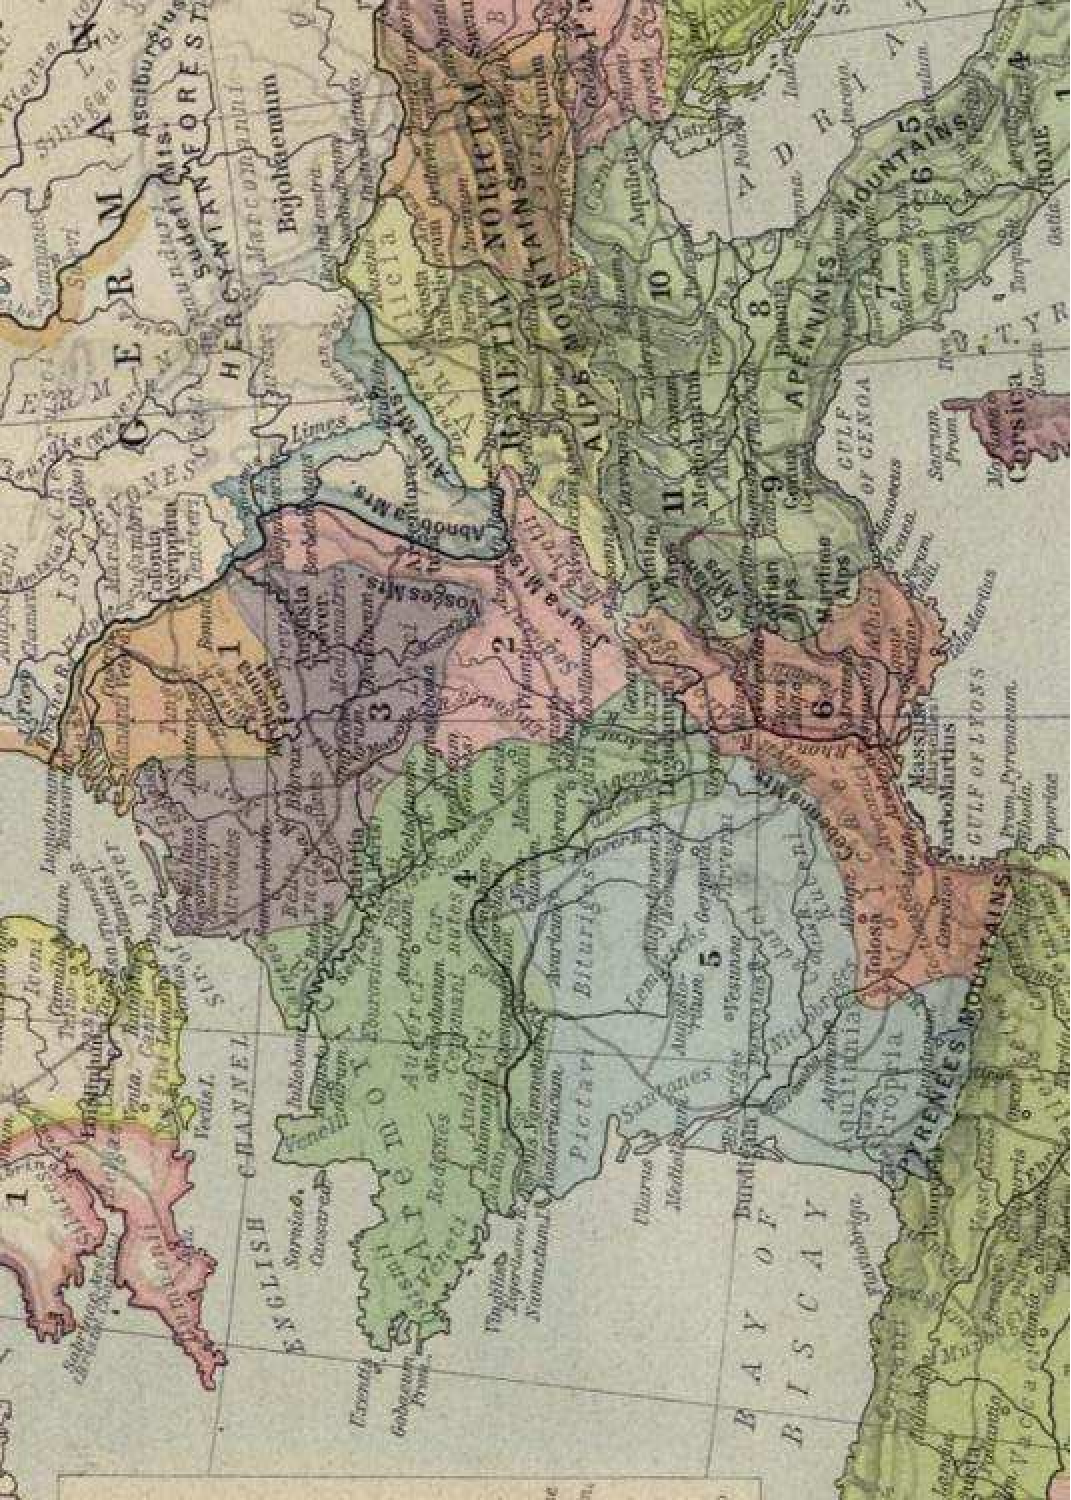
\includegraphics[width=175pt, angle=270]{bilder/Galia}
		\caption{Gallien zur Zeit Caesars}\label{fig_Gallien}
	\end{center}
\end{figure}


\begin{table}[htb]
	\begin{center}
		\begin{tabular}{|l|l|l|}
			\hline
			Jahr  & Erster Consul        & Zweiter Consul        \\
			\hline \hline
			1     & C. Caesar            & L. Aemilius Paullus   \\
			2     & P. Vinicius          & P. Alfenus Varus      \\
			3     & L. Aelius Lamia      & M. Servilius          \\
			4     & Sex. Aelius Catus    & C. Sentius Saturninus \\
			5     & L. Valerius Messalla & Cn. Cornelius Cinna   \\
			suff. & C. Vibius Postumus   & C. Ateius Capito      \\
			6     & M. Aemilius Lepidus  & L. Arruntius          \\
			\hline
		\end{tabular}
		\caption{Römische Konsulen}\label{tab_Konsulen}
	\end{center}
\end{table}


\pagebreak

\section{Background}
\subsection{Biology}
Cell line development is a process of generating single cell-derived clones that produce high and consistent levels of target therapeutic protein. (pharma.lonza.com/offerings/mammalian/cell-line-development)

Differential interference contrast (DIC) microscopy is an optical microscopy technique used to enhance the contrast in unstained, transparent samples (wikipedia).

Proteins are large biomolecules and macromolecules that comprise one or more long chains of amino acid residues (https://en.wikipedia.org/wiki/Protein).

Fluorescent labelling is the process of covalently binding fluorescent dyes to biomolecules such as nucleic acids or proteins so that they can be visualized by fluorescence imaging (https://www.nature.com/subjects/fluorescent-labelling). A fluorophore is a chemical compound that can reemit light at a certain wavelength.These compounds are a critical tool in biology because they allow experimentalists toimage particular components of a given cell in detail. (O'reilly life sciences p113)

Cell line development (CLD) is the process by which the cellular machinery is co-opted to manufacture therapeutic biologics or other proteins of interest. One can use different expression systems for cell line development: bacterial, plant-based, yeast, mammalian. (copy paste from https://www.beckman.de/resources/product-applications/lead-optimization/cell-line-development) Chinese hamster ovary (CHO) cells are the most popular mammalian cells used for protein production. (doi:10.1016/B978-0-08-100623-8.00007-4) 

First step of CLD is the
introduction of the gene of interest (GOI or a DNA vector) to CHO cells. This process is called a transfection. It is important to transfect a GOI into an optimal site of genome to secure a high protein expression over time during protein production, however pratically transfection mostly results in a vector being inserted into a random site within a host cell genome. In case the gene was transfected in the inactive site of genome (and the majority of genome is not transriptionally active) the cell will likely not express the gene. (doi:10.1016/B978-0-08-100623-8.00007-4) (doi:10.1016/j.coche.2018.08.002)

The second step is the selection of cell pools that have successful and stable gene integrations. The reasond why not all of them are suitable for cloning is the following: during the transfection only 80\% of cells recieve the vector of GOI (doi:10.1016/B978-0-08-100623-8.00007-4), only the small percent of which actually integrate a vector into the genome and, as mentioned above, only a fraction of those cells are able to stabily express a protein. (Reference needed). Such selection could be done with bulk sorting algorithm. (doi:10.1016/B978-0-08-100623-8.00007-4)

The third step in CLD is to clone the cells. The chosen stable pools of cells are phenotypically and genetically diverse - meaning they have different growth rates, metabolic profile and etc. This is not ideal for industrial production - all the cells used for protein production should be derived from the same clone ([25] here doi:10.1016/B978-0-08-100623-8.00007-4). In order to choose single best cells for further cloning one asseses several parameters like cell size, granularity, cell surface protein expression and etc. This can be done with Fluorescent Activated Cell Sorting (FACS) technology. (https://doi.org/10.1517/14712598.4.11.1821). Unfortunately fluorescence labeling is expensive and may ruin the cell due to its phototoxicity (https://doi.org/10.1371/journal.pone.0007497). There is a limited number of available fluorescent channels in microscopes as well as such labels can also be inconsistent, depend a lot on reagent quality, and require many hours of lab work. Therefore there exists a need for flurescent labeling in silico - without intervening into the cell. 

Once the cells are cloned, phenotypical and genetical heterogeneity is reduced, the next step is to charaterize clonally-derived cells based on the following criteria: cell size, growth rate, protein quality, titer, metabolities and etc. With this one can estimate clones productivity and titer. Such observations may take up to 90 days after which one can determine which cells are stable and therefore suitable for production. This is the last step of CLD process and consumes a lot of time and maintaining costs for feeding and cloning the cells. Predicting the stability of the cells directly from DIC images would reduce this time significantly allowing to escape this process completely.

However there are also some disadtantages of this approach. First, it can be less accurate than skilled cells staining perfomed manually. Extreme or unsual clones and phenotypes might be challenging if they were not used in the training set of images.

\subsection{Imaging}
The microscope used in the experiments takes photos of the well plate in random locations. The reason for that hides in the focusing problem, to get a reasonably good photo without blur it has to focus on a specific location, this is done there automatically, therefore the location of the focus is almost random. Although it might be problematic in the following sense: photos takes by the microscope in such manner do not gurantee that the focus will land in distinct spots all the time. This means that some cells taken during one of the photos might appear in the later ones. Since the photos have a high-resolution the crops are first performed and it might happen that same cell might appear in several crops. Afterwards, when crops are split between train, test and validation datasets it might happen that the same cell will once land in the train set and another time in the validation set, which will lead to a not completely fair and representative validaiton loss during training.

\subsection{ML}
Background on Unet and ML in general

Convoutional neural network is a neural network that is based on convolutional layers. It is a powerful tool for image processing and is used in medical imaging. Convolution is a linear operation used in convolutional layers that can be performed by applying a kernel (a 2d matrix) across a bigger input matrix called tensor, which can be 3d. Element-wise product between them is calculated and summed, this value will be an element of the output 2d matrix. Kernel slides accross all locations of the input tensor. In case if several different kernels were used then a 3d tensor will be created. 

Main advantage of convolutional neural networks if weight sharing. Kernel has learnable weights however these weights are shared across all locations of the kernel on the input tensor, thic strongly reduces the number of parameters needed.

CNNs also uses non-linearities like RELU, ELU, Tahn, Sigmoids and etc. They are also often combined with max pooling layers and dropouts to escape overfitting. 

Overfitting is one of the most often problems in deep learning that prevents model to generalize well for unseen data. This can happen when the model is too big for the amount of training data given, it was not regularized well or there is just not enough data for training. 

U-Net architecture is widely used for segmentation purposes. It is a convolutional neural network with the following architecture: [img] . It first performs image downsampling and upsampling afterwards.
[https://arxiv.org/pdf/1505.04597.pdf] The following architecture have been used for nuclei prediction. 
\begin{figure}[htb]
	\begin{center}
		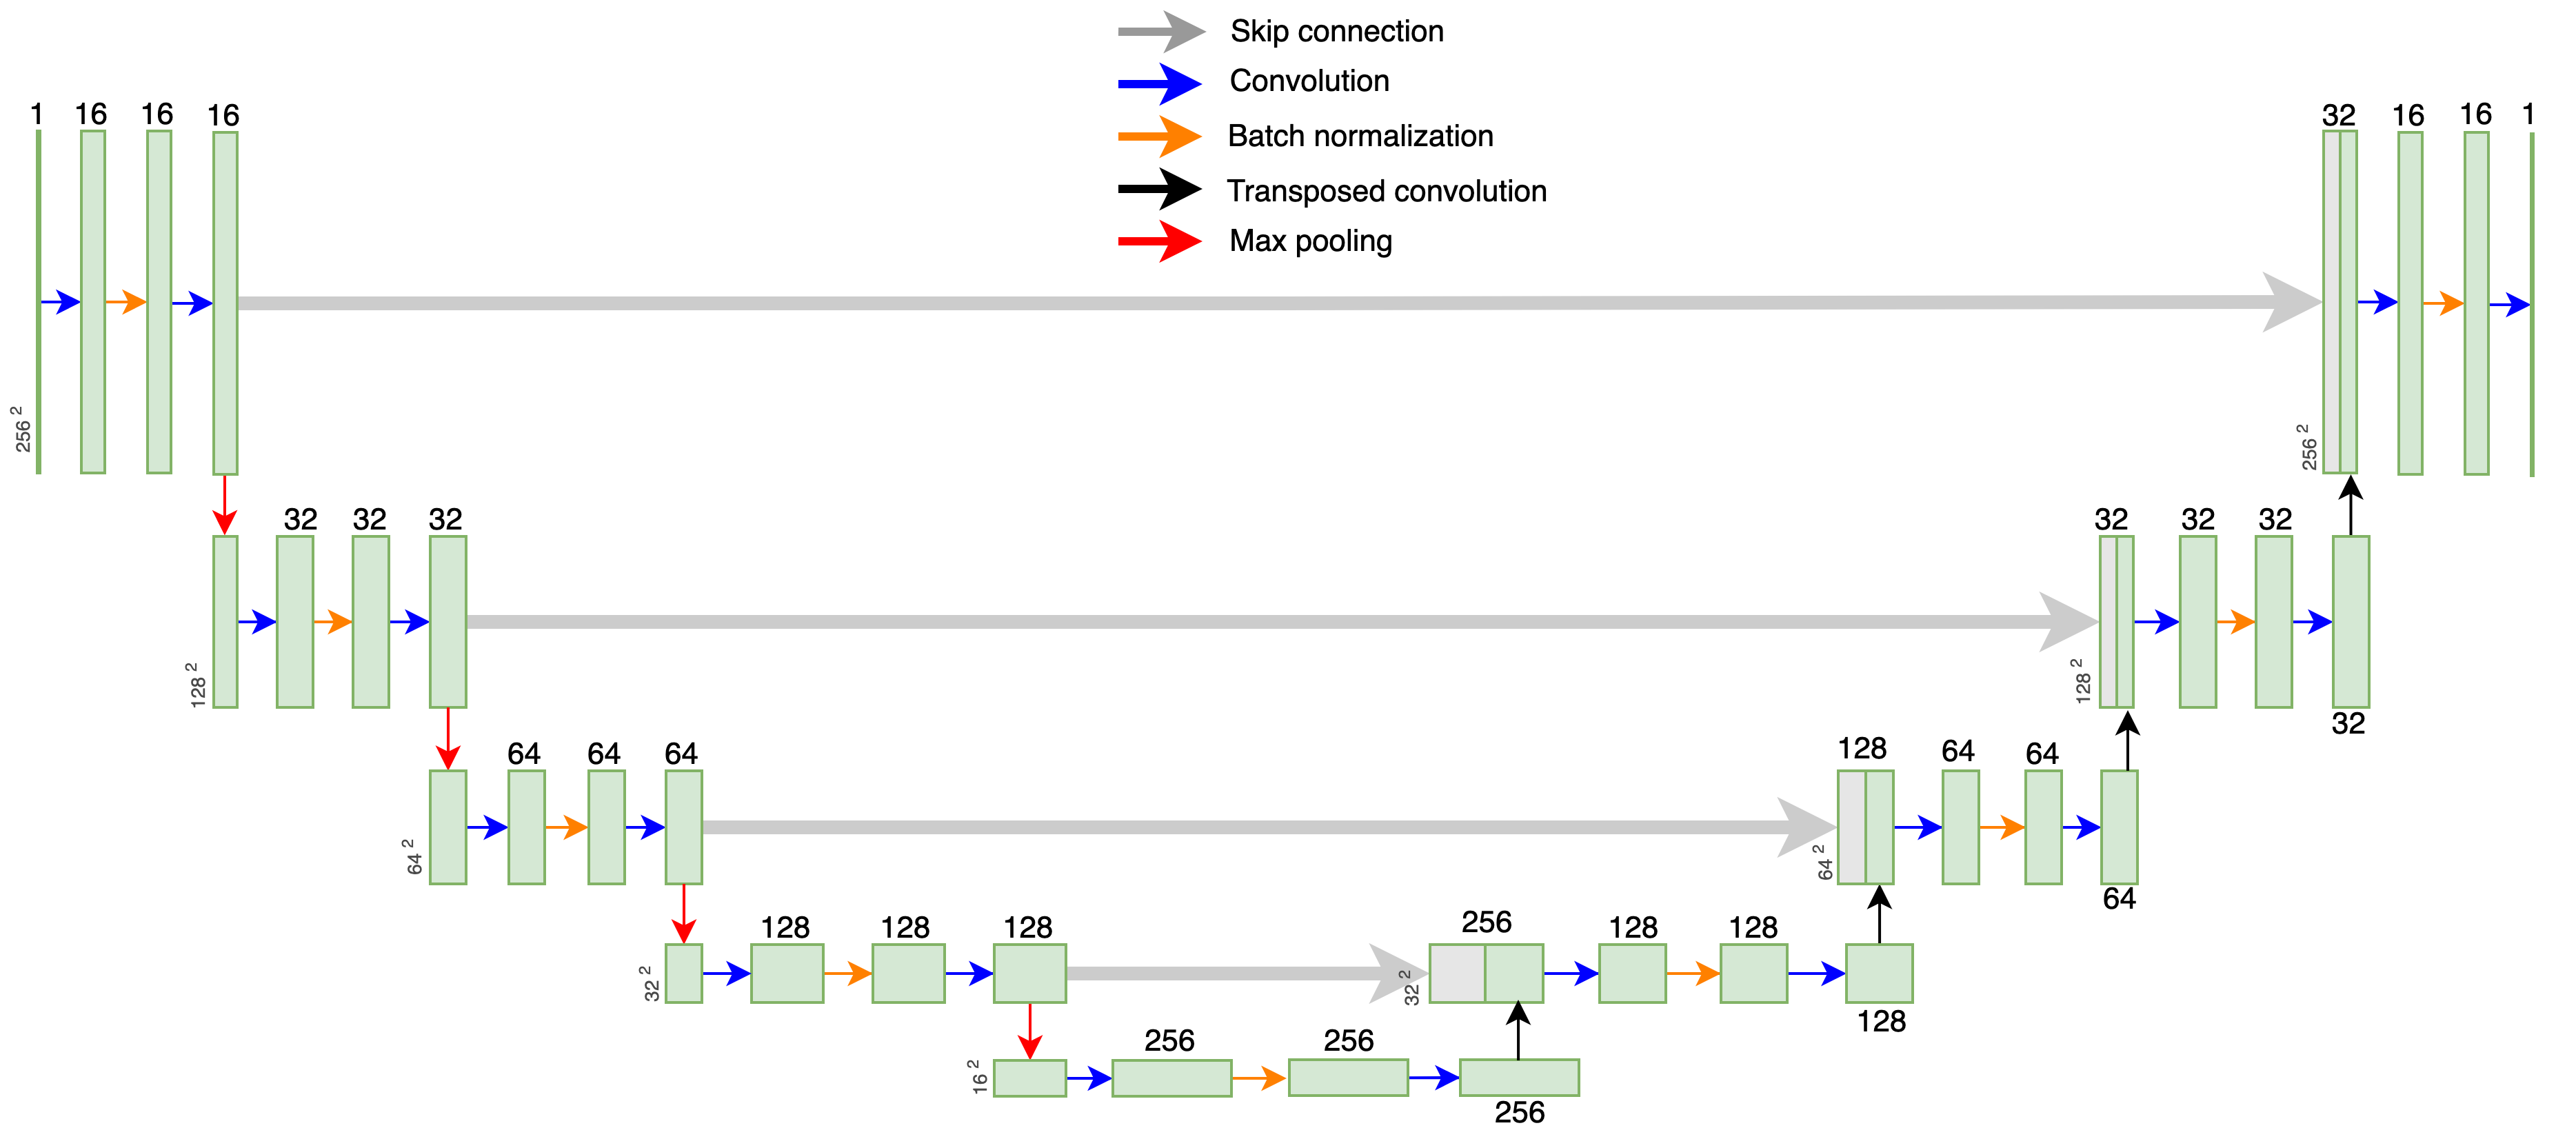
\includegraphics[width=\linewidth]{bilder/Unet.png}
		\caption{Unet}\label{fig:unet}
	\end{center}
\end{figure}

\section{Summary}
\subsection{Results}
\begin{itemize}
    \item In the scope of this master thesis three UNet models were developed that are able to predict fluorescence signal from DIC image data for the following targets: nuclei, endoplasmic reticulum and full cell surface. It was shown that developed models can successfully replace a manual fluorescence staining procedure as they are visually as well as based on practical biological metrics similar to the ground truth fluorescence images.
    
    \item Several adjustments before running any longer training experiment to model's training pipeline were made. First, the model's architecture from \cite{Lachance_2020} that was used in the experiments was improved in terms of faster learning with the use of batch normalization layers. Second, additional image augmentations like rotations and scaling were added and their logic was improved through the use of the high-resolution original image from the standard one. Third, the importance of a correct weight initialization was presented. And lastly, the model was tuned by choosing the correct regularization and optimization algorithms (batch normalization and adadelta optimization in this case). 
    
    \item For each of the four targets corresponding image preprocessing pipelines were developed. This step was very important to improve training data quality and address models' limitations before training, such as background-foreground class imbalance for instance. In the the Golgi apparatus preprocessing pipeline advanced methods like background removal using a rolling ball algorithm and image enhancement were introduced.
    
    \item In each training procedure, the model has successfully converged for all fluorescence targets except for the Golgi apparatus. Training experiments for the Golgi target showed that there is a lack of training data with high enough signal-to-noise ratio. Therefore further research can be carried out once the data with an improved signal-to-noise ratio has been collected, for example after a use of a better antibody for staining. However, several attems to improve model's predictions for the Golgi apparatus target were made via the use asymmentrical losses and advanced image preprocessing techniques. State-of-the-art papers like \cite{Cheng_2021} also demonstrate how challenging the Golgi predictions can be and therefore an accurate model for the Golgi apparatus predictions remain an open research challenge.
    
    \item The models' limitations in terms of intensity predictions were resolved. Based on visualizations and biological metrics estimations it was derived that the models have a similar downside in overpredicting total and mean intensities. Nevertheless, a strong correlation between the values suggests that there is an absolute value shift in predictions that can be fixed with relative ease. This issue was solved with the use of a bigger model and more data respectively. An immediate improvement was achieved when it comes to the correlation coefficients between the prediction and ground truth in the total and mean intensities.
    
    \item The models were evaluated against a set of common practical biological metrics including organelle quantity, total intensity, mean intensity and area of the organelle of interest. Every model was evaluated based on these metrics. It was shown that not only a significant correlation with ground truth values in terms of Pearson and Spearman rank correlation coefficients is present, but that the forms of distributions visualized with violin plots are very similar.
    
    \item For each organelle in question corresponding segmentation pipelines were developed, since the evaluation of the models on biological metrics require the segmentation of each predicted organelle. Postprocessing procedures for segmentation were successfully built with the OpenCV (\cite{opencv}) and \textit{skimage} (\cite{scikit}) libraries. 
    
    \item Generalizability study of the models across cell phenotypes and across not fixed cells was carried out. Regardless on which cell size was the model trained, it was able to generalize across different cell scales if the difference is under $30\%$. However, biological metrics show that intensities can be better reproduced when training on bigger cells. Lastly, an inductive bias of a model for full cell surface was determined: the model is able to select all the cells in the foreground regardless their state (both live and dead).

    \item Apart from generalizability models were tested on the stability of their predictions. For that goal artificially corrupted via image processing (like brightness, contrast changes and defocus blur imitations) data and data corrupted from faulty microscopy settings were introduced. It was shown that the models are very stable against changes in contrast and brightness, which can be caused by an over- or underexposure. Even though the models were very prone to errors with defocus blur corruption, using artificial corruptions as training augmentations improves models performance on corrupted images. Prediction on the image with corruptions created in the laboratory have shown that the models are stable against errors in cell fixation process, however they are quite sensitive towards errors in the focus of the microscope.
    
    \item UNet embeddings were studied for the possible source of additional data insights like phenotype differences or corruptions and unsupervised clustering algorithms were applied. The study has shown that image embeddings are not clustered based on cell phenotype, however corrupted images indeed form a separate cluster in the embeddings space. Nevertheless, this cluster is not well-separable from the rest of the data and further research is required. In an attempt to find a lower dimensional embedding for image representation an autoencoder embedding that was trained. The training has been carried out using the same data and the embeddings were checked for the same clustering targets. The results have shown strong clustering based on the brightness of the crops, which is not significant for this research as the brightness changes are very typical in DIC imaging due to slight differences in the exposure times and can be detecte with far easier methods.
    
    \item Finally, In order to detect corruptions and determine whether a models' prediction should or should not be reliable, two drift detection algorithms were developed. The first one is based on the maximum mean discrepancy method, and the second one is an online version of the first one. They were tested on both corruption types and have shown strong ability for detecting drift in data with high ROC-AUC scores. These algorithms performed much better than the clustering approach mentioned above and can be used in practice.
\end{itemize}
%Intensity fluorescence predictions as well as binary segmentation (for the full cell surface target) were visualized. 

\subsection{Limitations}
The main limitation of this research is the need to fix the cells before taking DIC images of them. Cell fixation is a preceding step before cell staining --- therefore all cells in datasets of DIC images were fixed. Since living and fixed cells look very different and models trained on fixed cells do not generalize to non-fixed ones well, predictions can be carried out on DIC images of fixed cells only. Luckily, fixing procedure is not a cumbersome lab procedure and is far easier than staining the cells, which is avoided with the help of \textit{in-silico} fluorescence labeling. It is recommended to look into possibilities of transfer learning from fixed to living cells. 
Also, models developed here cannot generalize well on other cells apart from CHO and are able to produce accurate predictions for the cells used in this laboratory only. However, in future the developed product would aim to address the specific needs of each laboratory separately. Therefore the models will be trained with the goal to address the issues of one specific cell line. 


\subsection{Future research}
This research sets the ground for a variety of further research ideas:
\begin{itemize}
    \item As the Golgi apparatus model did not produce good enough predictions due to several reasons (such as low signal-to-noise ratio in input data, as well as an extremely strong class imbalance between the foreground and background in images), it is strongly recommended to continue research in this direction. For example, by choosing another target protein in the staining procedure, applying stronger noise reduction approaches as introduced by \cite{noise2void}, and incorporating image gradients in the loss function.
    \item UNet embeddings do indeed show a potential for detecting corruptions in crops, however it is not strong enough. It is highly recommended to incorporate embeddings of all crops from the same image into one point in the embedding space. For example, by averaging the embeddings. This might show a more significant clustering of corrupted data.
    \item Since autoencoder embeddings have shown clear clustering based on the crop brightness, it would be beneficial to normalize the brightness across all crops first. This would allow an autoencoder to pay attention to other less distinctive features in the image. However, due to the non-uniform distribution of the cells in the image this approach not the most promising one.
    \item Drift detction can also be implemented based on raw DIC input without involving model's predictions at all. Therefore it is recommended to further drive research in the direction of contrastive learning algorithms for out of distribution detection, specifically following the approach proposed by \cite{csi}.
    \item Due to time constraints it was not possible to train very big models, however the improvement of prediction quality that occurs after a model enlargement is very significant. Therefore if the higher image resolution is needed, it is recommended to train models with a bigger model size and more data.
    \item The lack of data concerning corruptions from the microscopy settings did not allow to test online drift detection algorithm. As this version very promising for practical use it is recommended to use more data for its testing.
    \item Since the model for full cell surface predictions is not able to distinguish between dead and live cells, it is recommended to add more images that include dead cells into the dataset or to train an alternative model that is able to distinguish them (\cite{Ounkomol_2018}).
    \item Although staining several organelles can be challenging due to the chemical reactions between fluorophores, staining multiple organelles at the same time would provide a possibility to train the model to predict several organelles at the same time.  while sharing mutual information between them.
\end{itemize}
 
Advances of AI and deep learning are a promising direction for the future of the field of cell line development. This work serves as evidence of the progress allowing to reduction time and cost of manual work in biological laboratories. The automation of one step of the cell line development was shown in this research, but there are many more prospects regarding the use of deep learning for the development of more automated cell line development systems. Specifically, for predicting cell stability and productivity, which is the general goal of the Merck KGaA's project, within which this study was carried out. The use of the models developed here can potentially bring useful feature representations that can be incorporated into the pipeline for productivity predictions and save reduce the time spent on manual work even more.

\pagebreak
\section{Weiteres Kapitel}\raggedbottom
\subsection{Unterkapitel}
\subsection{Unterkapitel}

%%%%%%%%%%%%%%%%%%%%%%%%%%%%%%%%%%%%%%%%%%%%%%%%%%%%%%%%%%%%%%%%%%%%%%%%
%%%% ENDE TEXTTEIL %%%%%%%%%%%%%%%%%%%%%%%%%%%%%%%%%%%%%%%%%%%%%%%%%%%%%
%%%%%%%%%%%%%%%%%%%%%%%%%%%%%%%%%%%%%%%%%%%%%%%%%%%%%%%%%%%%%%%%%%%%%%%%

\clearpage

% Entfernen Sie das Kommentar aus der nachfolgenden Zeile, falls Sie einen Anhang in der Arbeit verwenden wollen. Beachten Sie, dass Sie sich im Verlauf der Arbeit mit \ref{...} (z.B. \ref{anhang:zusatz1}) auf den Anhang beziehen.
%\newpage
\appendix
\section{Anhang}

\subsection*{Zusatzteil 1} \label{anhang:zusatz1}

Dies ist ein Anhang.

\clearpage

\ifthenelse{\boolean{\biber}}{ %with biber do
	\DeclareNameAlias{sortname}{first-last}
	\printbibliography[heading=bibintoc, title=\references]
}{ %without biber do
	\bibliography{references}
	\bibliographystyle{alphadin}
}
%\vspace*{\fill}

\clearpage

\listoffigures

\listoftables

%\pagebreak

%\printindex
\end{document}
